\section{Measurement Technique}
\begin{frame}{Measurement principle: Coulomb explosion + VMI readout}
\small
\begin{itemize}
  \item \textbf{Prepare:} Molecules are embedded in $^4$He nanodroplets and are aligned/spun up by the pump
        (e.g.\ optical centrifuge) at a controlled pump--probe delay.
  \item \textbf{Coulomb explosion (probe):} A short, intense probe pulse removes multiple electrons
        $\Rightarrow$ the molecule becomes a \textbf{highly charged ion} and fragments.
  \item \textbf{Axial recoil:} Fragment ions recoil mainly along the \textbf{molecular bond axis}
        (for suitable channels) $\Rightarrow$ ion emission angles encode the instantaneous molecular orientation.
  \item \textbf{Velocity Map Imaging (VMI):} Electrostatic lenses map the 3D ion velocity distribution onto a 2D detector:
        ions with the same transverse velocity hit the same detector radius.
  \item \textbf{Detection \& analysis:} The detector image (MCP/phosphor + camera) gives
        \textbf{angular distributions} (alignment/orientation) and \textbf{kinetic energy release};
        repeating vs delay reconstructs the rotational dynamics.
\end{itemize}
\end{frame}
\begin{frame}{Example of one measurement frame}
\small
\begin{minipage}[c]{0.5\textwidth}
  \centering
  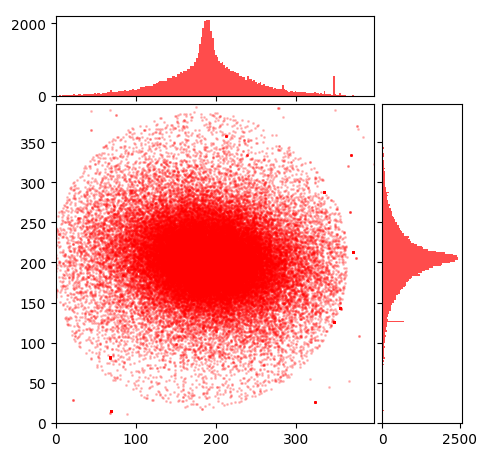
\includegraphics[width=.65\linewidth]{pic/ions_unprocessed.png}
  \captionof{figure}{Detected ions (unprocessed)}
\end{minipage}\hfill
\begin{minipage}[c]{0.5\textwidth}
  \centering
  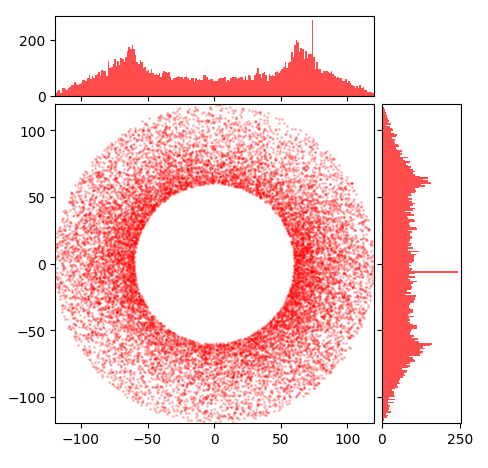
\includegraphics[width=.65\linewidth]{pic/ions_processed.png}
  \captionof{figure}{Detected ions (processed)}
\end{minipage}
\begin{itemize}
      \item We scan the pump--probe delay
        \[
          \tau = t_{\mathrm{probe}} - t_{\mathrm{pump}}
        \]
        to map the time-dependent rotational dynamics.
\end{itemize}
\end{frame}